\chapter{Machine Learning}\label{chp:ml}

\section{Tratamento dos dados}\label{sec:data1}

\subsection{Dados obtidos da UCI}
	Para grande parte dos testes de  \textbf{\textit{Cross-Validation}}, foi usado um dataset obtido por meio do reposit�rio online da UCI. 
	
	
\subsection{Dados do Servidor}	






\section{Formato dos dados tratados}
A matriz de dados tratados usada diretamente pelos algoritmos de ML tem o seguinte formato:


\begin{blockarray}{cccccc}
$ZoneID$ & $BSSID_1$ & $BSSID_2$ & ... &  $BSSID_n$ \\
\begin{block}{(ccccc)c}
  1&-70 & -92 &   ... &-87&  $ Measure_1$ \\
  2&-89 & -80 & ... & -63&    $Measure_2 $\\
  3&-28 & -120 & ...&   -35& $Measure_3$ \\
   \vdots& \vdots &  \vdots & $\ddots$ &  \vdots &    \vdots \\
  1&-48 & -36 & ... &   -29&  $Measure_n$ \\
\end{block}
\end{blockarray}
 


\centerline{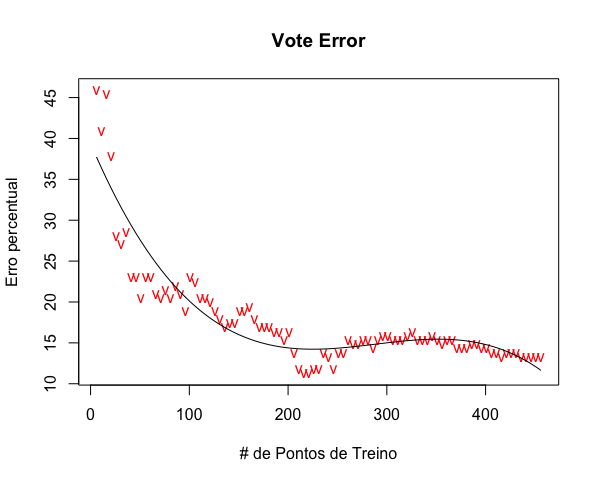
\includegraphics[scale=.55]{VoteError2zonesUCI}}